\documentclass{article}
\usepackage[utf8]{inputenc}
\usepackage[polish]{babel}
\usepackage[T1]{fontenc}
\usepackage{multicol}
\usepackage{multirow}
\usepackage{amsmath}
\usepackage[export]{adjustbox} 
\usepackage{float}
\usepackage{graphicx}
\usepackage{chngpage}
\usepackage{longtable}
% table struts
\usepackage{listings}
\usepackage{layout}

\usepackage{caption}
\usepackage{rotating}
\usepackage{geometry}
%  \usepackage{draftwatermark}
%\SetWatermarkText{DRAFT}
%\SetWatermarkScale{5}
\usepackage{lscape}
\newcommand\T{\rule{0pt}{2.6ex}}       % Top strut
\newcommand\B{\rule[-1.2ex]{0pt}{0pt}} % Bottom strut
\usepackage{array}   % for \newcolumntype macro
\newcolumntype{L}{>{$}l<{$}} 
\begin{document}
	
	\begin{titlepage}
		
		
		
		\vspace{5cm}
		
		\begin{center}
			\vspace*{1cm}
			
			{\Huge \textbf{Optymalne sterowanie warunkiem brzegowym z wykorzystaniem metody Adjoint}}
			
			\vspace{0.5cm}
			{\huge Projekt 13}
			
			\vspace{1.5cm}
			\large{Filip Hahs}
			
			
		\end{center}
		\vfill
		
		
	\end{titlepage}
	\section{Problem}
Celem projektu było napisanie programu znajdującego taki rozkład temperatury zewnętrznej na brzegu $\Gamma_2$ w każdej chwili, aby rozkład temperatury w przestrzeni $\Omega$ był maksymalnie jednorodny. Na krawędziach należących do $\Gamma_1$ zadany jest adiabatyczny warunek brzegowy. 
\begin{figure}[H]
	\centering
	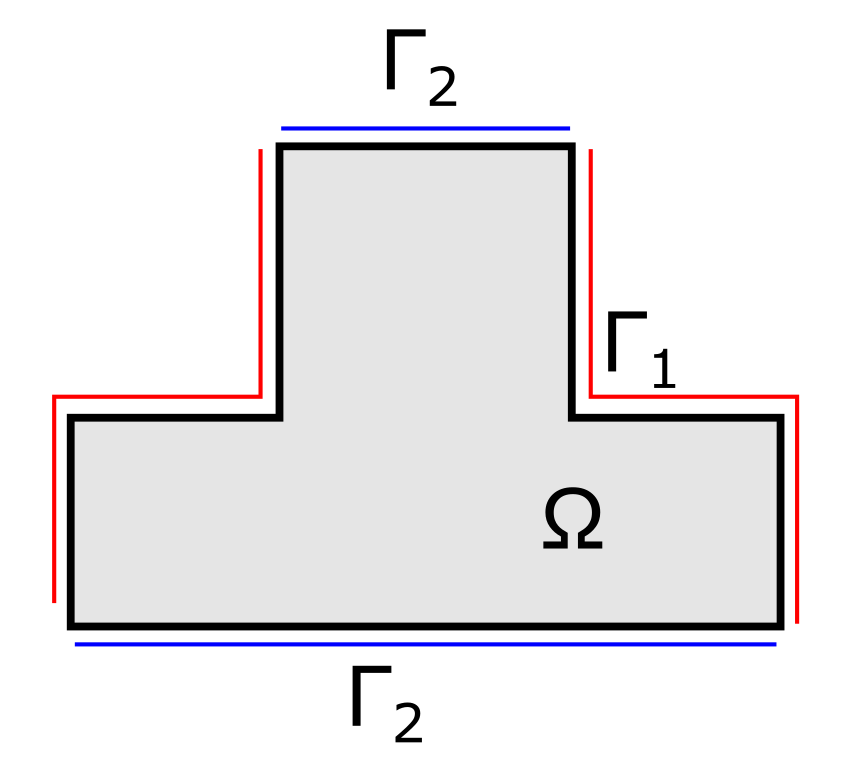
\includegraphics[width=0.5\linewidth]{plyta}
	\caption{Przestrzeń obliczeniowa}
	\label{fig:plyta}
\end{figure}
Równanie różniczkowe cząstkowe ma postać:
\begin{align*}
	\begin{cases}
		\frac{\partial u}{\partial t} = D\Delta u\; \text{dla}\; u\in\Omega\\
		D\frac{du}{dn} = \beta(c-u) \; \text{dla}\; u\in\Gamma_2\\
		\frac{du}{dn} = 0 \; \text{dla}\; u\in\Gamma_1\\
	\end{cases}
\end{align*}
gdzie:
\begin{align*}
	&D \text{ - to dyfuzyjność (przewodność cieplna)}\\
	&\beta \text{ - to współczynnik przyjmowania ciepła na brzegu}\\
	&c \text{ - to temperatura zewnętrzna - zmienna sterowana}
\end{align*}	
\end{document}